\section{State of the Art}
Grob betrachtet beinhalten verlustbehaftete Kompressionen drei Teilschritte: Transformation, Quantisierung und Entropie Kodierung. Die Abbildung \ref{state:aufbau} zeigt eine vereinfachte Abfolge. Die Inputdaten werden zuerst duch ein oder mehrere Verfahren transformiert. So transformieren, dass in der Quantisierung unwichtige Informationen entfernt werden können. Oft gehen nur im Quantisierungsschritt Daten verlohren, während alle anderen Schritte verlustfrei umkehrbar sind. Danach werden die Daten Entropie Kodiert. Für jeden Teilschritt gibt es unterschiedliche Verfahren. So können auch mehrere Transformationen hintereinander durchgeführt werden, oder eine ganze Folge von Transformations- und Quantisierungsverfahren.\\
\begin{figure}[!htbp]
	\center
	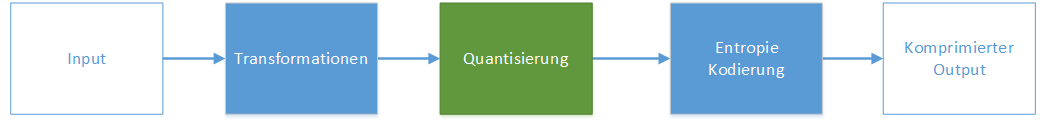
\includegraphics[width=0.8\textwidth,height=6cm,keepaspectratio]{./pictures/state/aufbau.png}
	\caption{Typische Teilschritte einer Kompression}
	\label{state:aufbau}
\end{figure}

\subsection{JPEG/JFIF Bildkompression}
\begin{figure}[!htbp]
	\center
	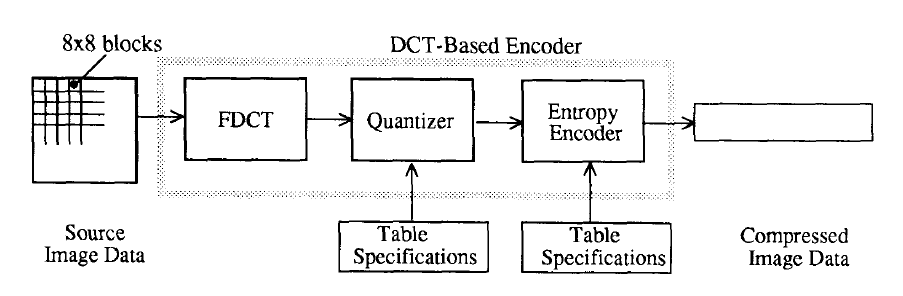
\includegraphics[width=0.8\textwidth,height=6cm,keepaspectratio]{./pictures/state/jpeg.png}
	\caption{Aufbau der JPEG Kompression \cite{wallace1992jpeg}}
	\label{state:jpeg:abb}
\end{figure}
Das JPEG/JFIF Bildformat ist eines der meist-verwendeten Bildkompressionsverfahren für natürliche Bilder. Das Diagramm der Abbildung \ref{state:jpeg:abb} zeigt den Aufbau der Kompressionspipeline. JPEG/JFIF unterteilt das Eingabebild in $8*8$ Blöcke und führt auf ihnen eine Diskrete Kosinus Transformation (DCT) durch. Der Bildblock ist nun als Folge von Kosinus-Funktionen dargestellt.\\
Die Quantisierung versucht nun Frequenzen, welche das menschliche Auge schlecht erkennen kann mit weniger Präzise darzustellen. Wenn die Quantisierung gut gewählt wurde, kann der Mensch das dekomprimierte Bild nicht vom Original unterscheiden, verbraucht aber weniger Speicherplatz. JPEG/JFIF bietet vorgefertigte Quantisierungstabellen an. Der Benutzer kann aber eigene Tabellen für spezifizieren. Wie die Quantisierungstabelle optimal gewählt wird, ist ein aktives Forschungsfeld \cite{wu1993rate:jpeg} \cite{wang2001designing:jpeg} und kann von Anwendungsfall zu Anwendungsfall unterschiedlich sein.\\
Nach der Quantisierung werden die quantisierten Blöcke im Zick-Zack-Muster angeordnet, sodass die Entropie Kodierung eine bessere Kompression durchführen kann. JPEG/JFIF führt eine Run-Length und eine Huffman-Kodierung durch. JPEG bietet auch hier an, eine benutzerspezifizierte Huffman-Tabelle zu verwenden.

Auf wissenschaftliche Floating-Point Daten

\subsection{Point Cloud Kompression}
\begin{figure}[!htbp]
	\center
	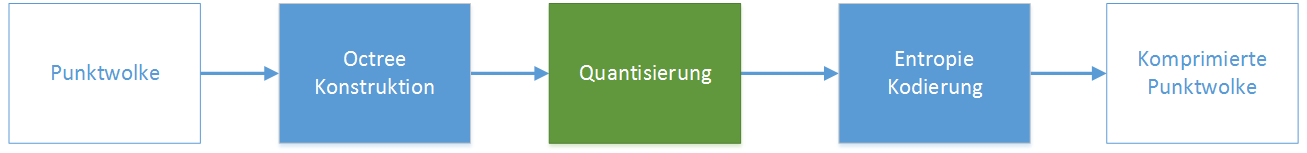
\includegraphics[width=0.8\textwidth,height=6cm,keepaspectratio]{./pictures/state/pointcloud.png}
	\caption{Aufbau einer Octree basierten Point Cloud Kompression.}
	\label{state:pointcloud:abb}
\end{figure}
3d Laser Sampling Geräte produzieren grosse Mengen an volumetrischen Punkten von alltäglichen Objekten. Die Kompression von solchen Punktwolken ist ein aktives Forschungsfeld. Eine vorgeschlagene Kompression  von Schnabel und Klein \cite{schnabel2006octree} verwendet Octrees \cite{wiki:octree}. Das Diagramm der Abbildung \ref{state:pointcloud:abb} verdeutlicht den Ablauf.\\
Die dreidimensionalen Punkten werden in einem Octree mit einer begrenzten Anzahl an Levels abgelegt. Im Quantisierungsschritt werden die Punkte durch die Zellenmittelpunkte des Octrees ersetzt. Die Anzahl an Levels ist gleichzusetzen mit der Genauigkeit in Bits welche für jede Koordinatenachse zur Verfügung stehen. Wenn die Levels auf $8$ begrenzt sind, steht für jede Achse $8$ Bit Genauigkeit zur Verfügung.\\
In der Entropie Kodierung wird der Octree zuerst mit einem Prediktiven und danach mit einer Arithmetischen Kodierung versehen. In der Prediktiven Kodierung liegt die Komplexität und die Güte der Kompression.\\

Je nach Implementation können zu jedem Punkt zusatzinfos gespeichert werden wie Farbe/Normalen etc, darüber könnte die Information, zu welcher Linie ein Punkt gehört, gespeichert werden.

\subsection{Curve Fitting}
Curve Fitting ist ein Teilgebiet der Signalverarbeitung. Ein Signal wird aus einer oder mehreren Basisfunktionen ausgedrückt und findet typischerweise Anwendungen in den Bereichen Signalinterpolation, Differenzierung und Rauschunterdrückung. Aber auch eine verlustbehaftete Kompression ist Möglich.

 Die B-Spline Transformation \cite{unser1993b:spline} ist in linearer Zeit. Möglichkeit, ein Signal mit B-Splines zu approximieren. Die Problematik liegt in den Details wie Anzahl Funktionen, Verteilung der Spline Knotenpunkten etc.

\subsection{Entropie Kodierung}
Die Entropie Kodierung findet in allen Bereichen der Informatik Anwendungen. Allgemeien Verfahren RLE, Huffman, Arithmetic

Fix fertige Pakete wie Gzip, Rar welche meist mehrere Verfahren kombinieren.

Spezialisierte Entropie Kodierun:Fast Lossless floating point compression \cite{ratanaworabhan2006fast}